\section{Financial network topology}
\label{sec:networks}

Clustering summarises hierarchical organisation, but it does not identify graph-theoretic hubs, bridges or local cycles. Financial networks provide these complementary views by retaining only the strongest distance-ranked edges under structural constraints. We therefore move from dendrograms to filtered financial networks to study how dependency topology changes after RMT filtering.

\subsection{MST backbone}

The MST is the sparsest connected representation of the dependency geometry. With $N=58$, it contains 57 edges. Figure~\ref{fig:mst_refined} compares the MST built from the original matrix with the MST built from the group-mode matrix. This comparison is useful because it shows how much of the original backbone is driven by the market mode.

\begin{figure}
\centering
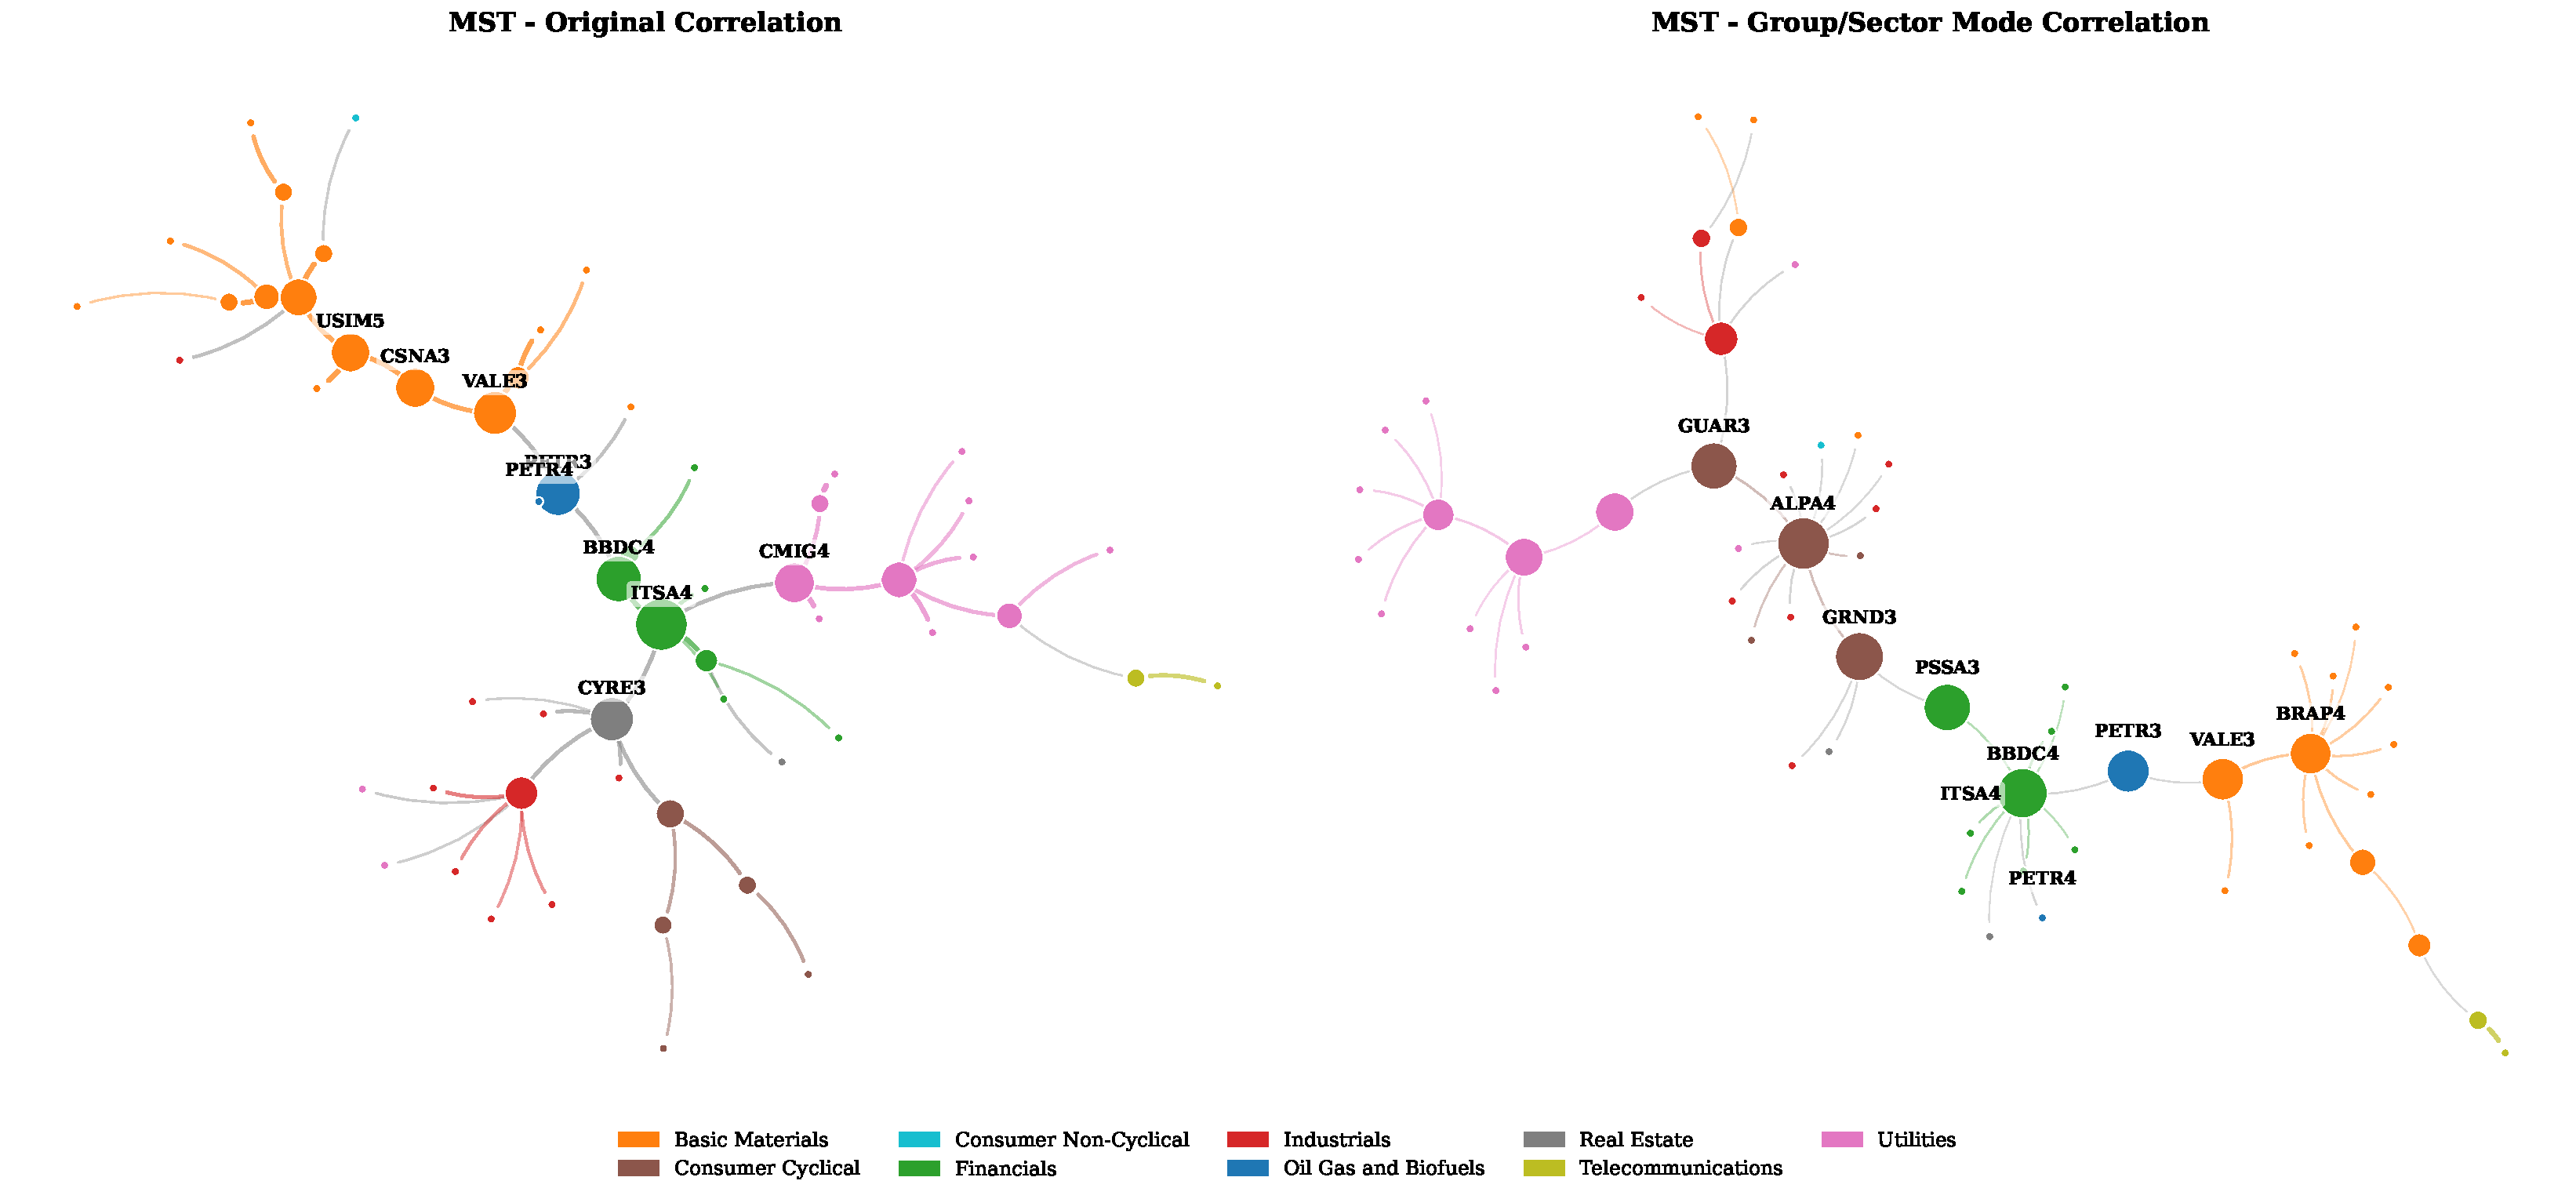
\includegraphics[width=\linewidth]{images/figure_11b_mst_refined_comparison.pdf}
\caption{Refined MST comparison for original and group-mode correlation matrices. The original MST emphasizes strong market-mode dependencies, while the group-mode MST highlights weaker localized dependency channels.}
\label{fig:mst_refined}
\end{figure}
\FloatBarrier

The original MST has mean edge correlation 0.5796, while the group-mode MST has mean edge correlation 0.1388. This large decline is expected because the group-mode network excludes the dominant common component. The same-sector edge ratio also changes, from 0.7193 in the original MST to 0.6316 in the group-mode MST. The group-mode MST is therefore not a weaker version of the original tree; it is a different view of the market after broad synchronization is removed.

\subsection{PMFG topology}

The PMFG is richer than the MST because it preserves planarity while retaining $3N-6=168$ edges. It therefore includes cycles, triangles and 4-cliques. Figure~\ref{fig:pmfg_refined} compares original and group-mode PMFGs. This is the main network visualization in the paper because the PMFG retains enough structure to study local communities and hub reorganization.

\begin{figure}
\centering
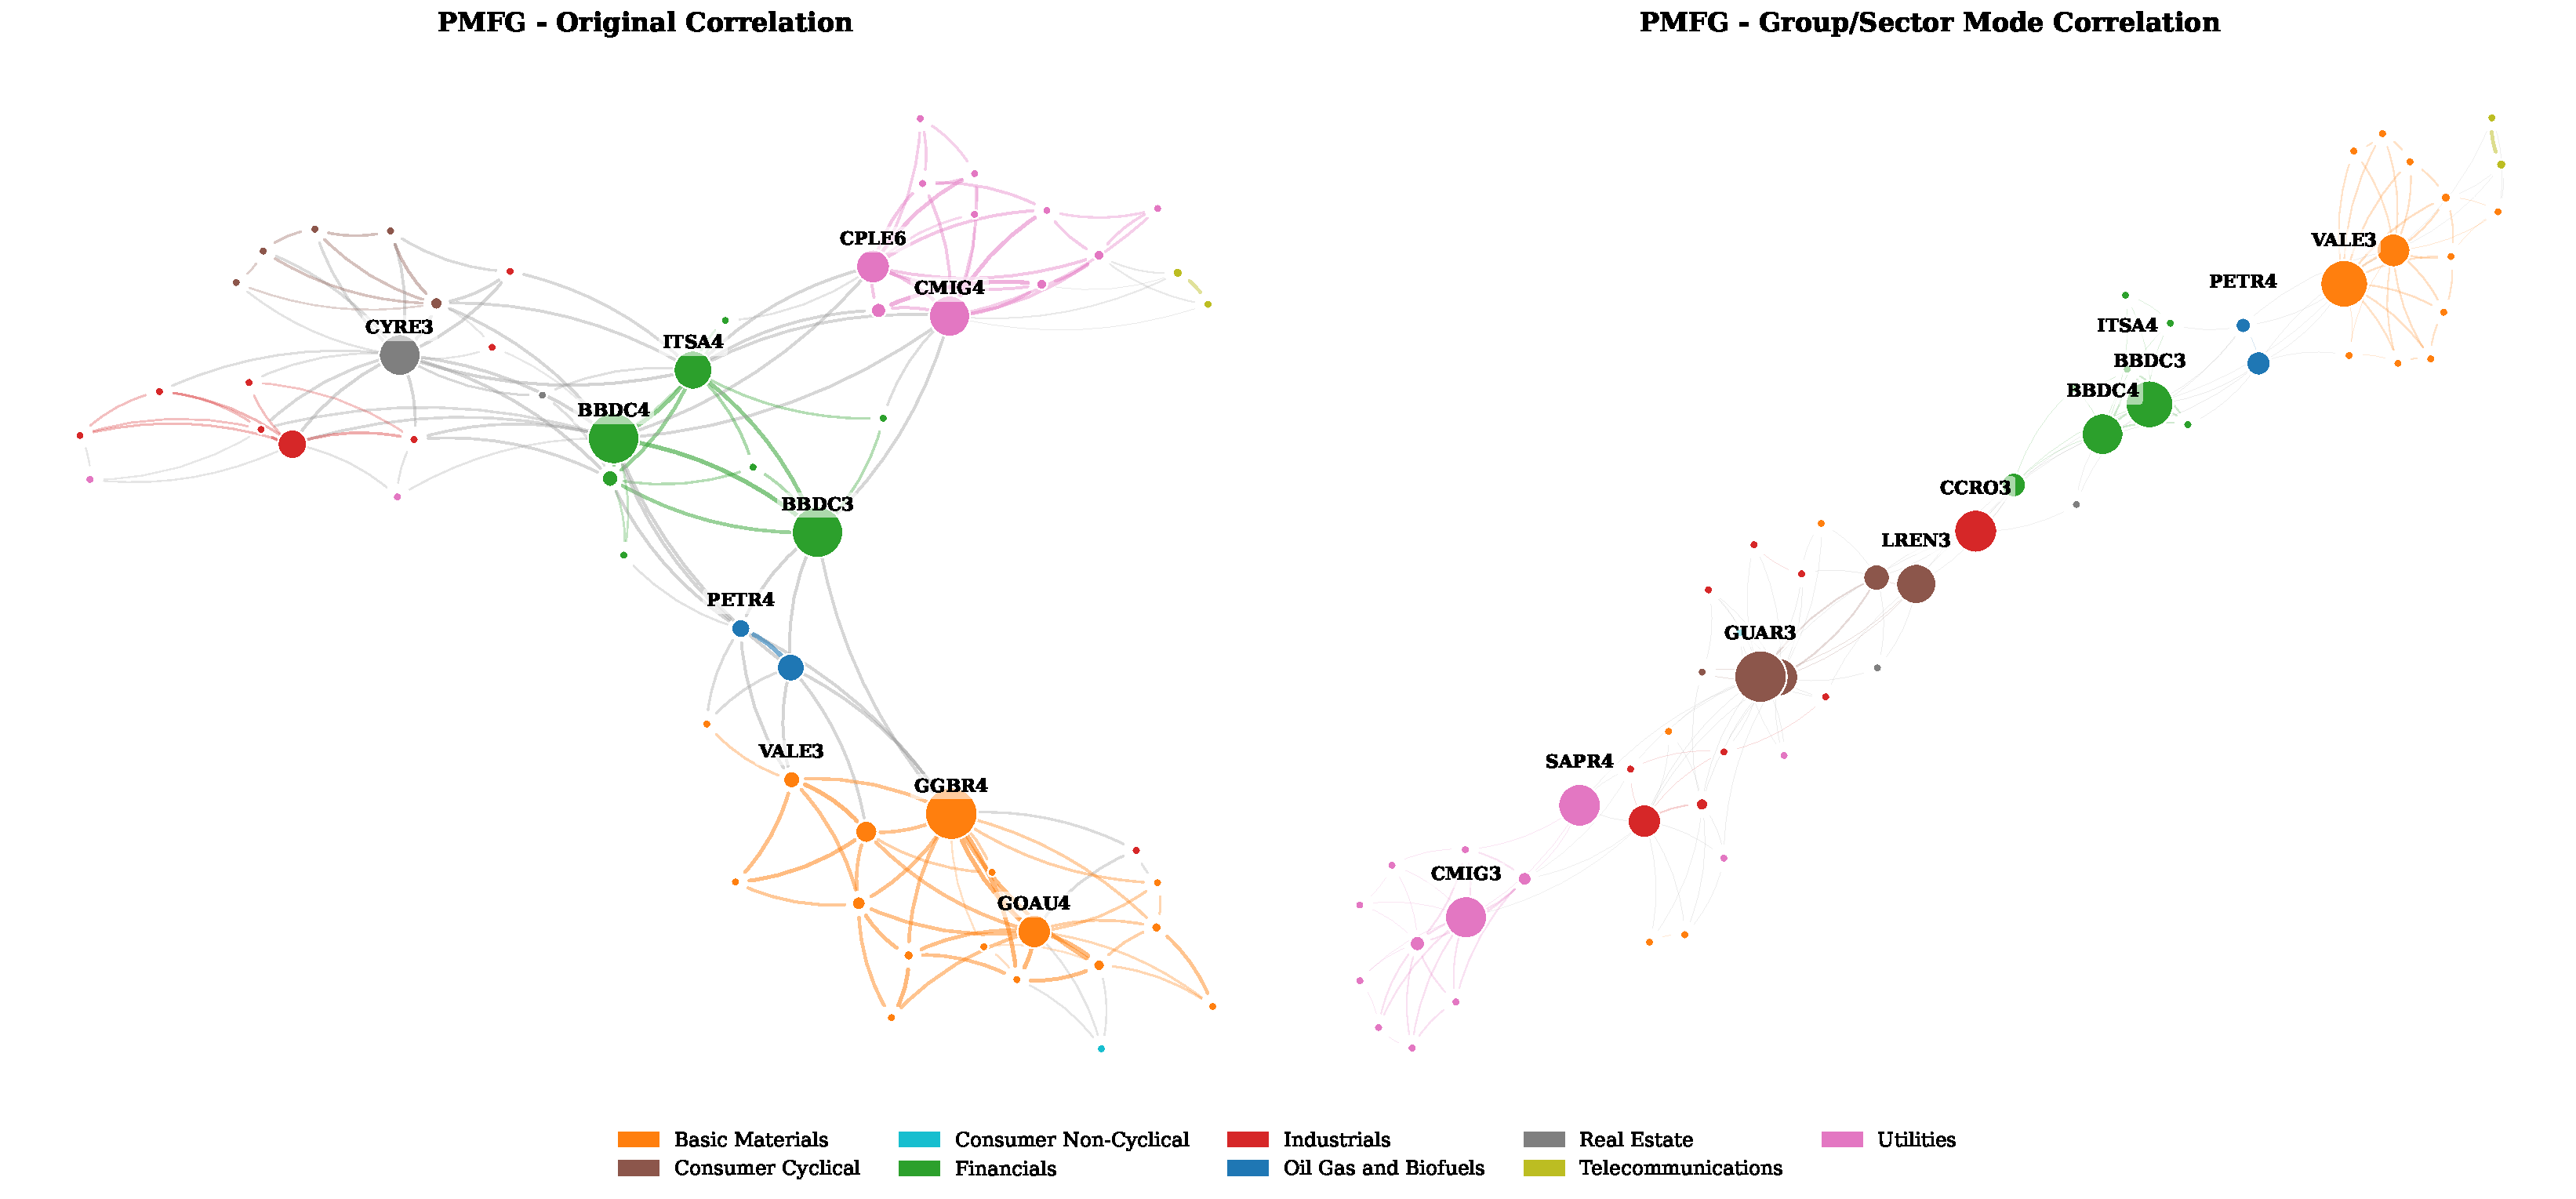
\includegraphics[width=\linewidth]{images/figure_12b_pmfg_refined_comparison.pdf}
\caption{Refined PMFG comparison for original and group-mode correlation matrices. The group-mode PMFG reduces market-wide dominance and highlights more localized dependency channels.}
\label{fig:pmfg_refined}
\end{figure}
\FloatBarrier

The original PMFG has mean edge correlation 0.5177. The group-mode PMFG has mean edge correlation 0.1109. Despite this lower average edge strength, the group-mode PMFG has higher average clustering, 0.6653, than the original PMFG, 0.5273. This is a central result: removing the market mode lowers the absolute level of edge correlations, but it can reveal more clustered local structure.

\subsection{Original vs Group/Sector Mode networks}

Table~\ref{tab:network_summary} summarizes the main MST and PMFG statistics. It shows the same pattern across graph families. Original networks have stronger edges because they contain the market mode. Group-mode networks have weaker edges but preserve meaningful sectoral and subsectoral organization.

\begin{table}
\centering
\caption{Selected MST and PMFG topology statistics.}
\label{tab:network_summary}
\resizebox{\linewidth}{!}{%
\begin{tabular}{llrrrrrrr}
\toprule
Network & Matrix & Edges & Mean edge corr. & Same-sector ratio & Clustering & Top degree & Top betweenness & 4-cliques \\
\midrule
MST & Original & 57 & 0.5796 & 0.7193 & 0.0000 & RAPT4 & ITSA4 & 0 \\
MST & Group mode & 57 & 0.1388 & 0.6316 & 0.0000 & ALPA4 & ALPA4 & 0 \\
PMFG & Original & 168 & 0.5177 & 0.6012 & 0.5273 & BBDC4 & GGBR4 & 55 \\
PMFG & Group mode & 168 & 0.1109 & 0.5417 & 0.6653 & GUAR3 & GUAR3 & 55 \\
\bottomrule
\end{tabular}}
\end{table}
\FloatBarrier

\subsection{Network topology metrics}

Figure~\ref{fig:network_topology} expands the comparison beyond average edge correlation. It summarizes mean edge correlation, same-sector ratio, same-subsector ratio and average clustering across network and matrix types. This figure is useful because it shows that topology is not reducible to a single edge-weight statistic.

\begin{figure}
\centering
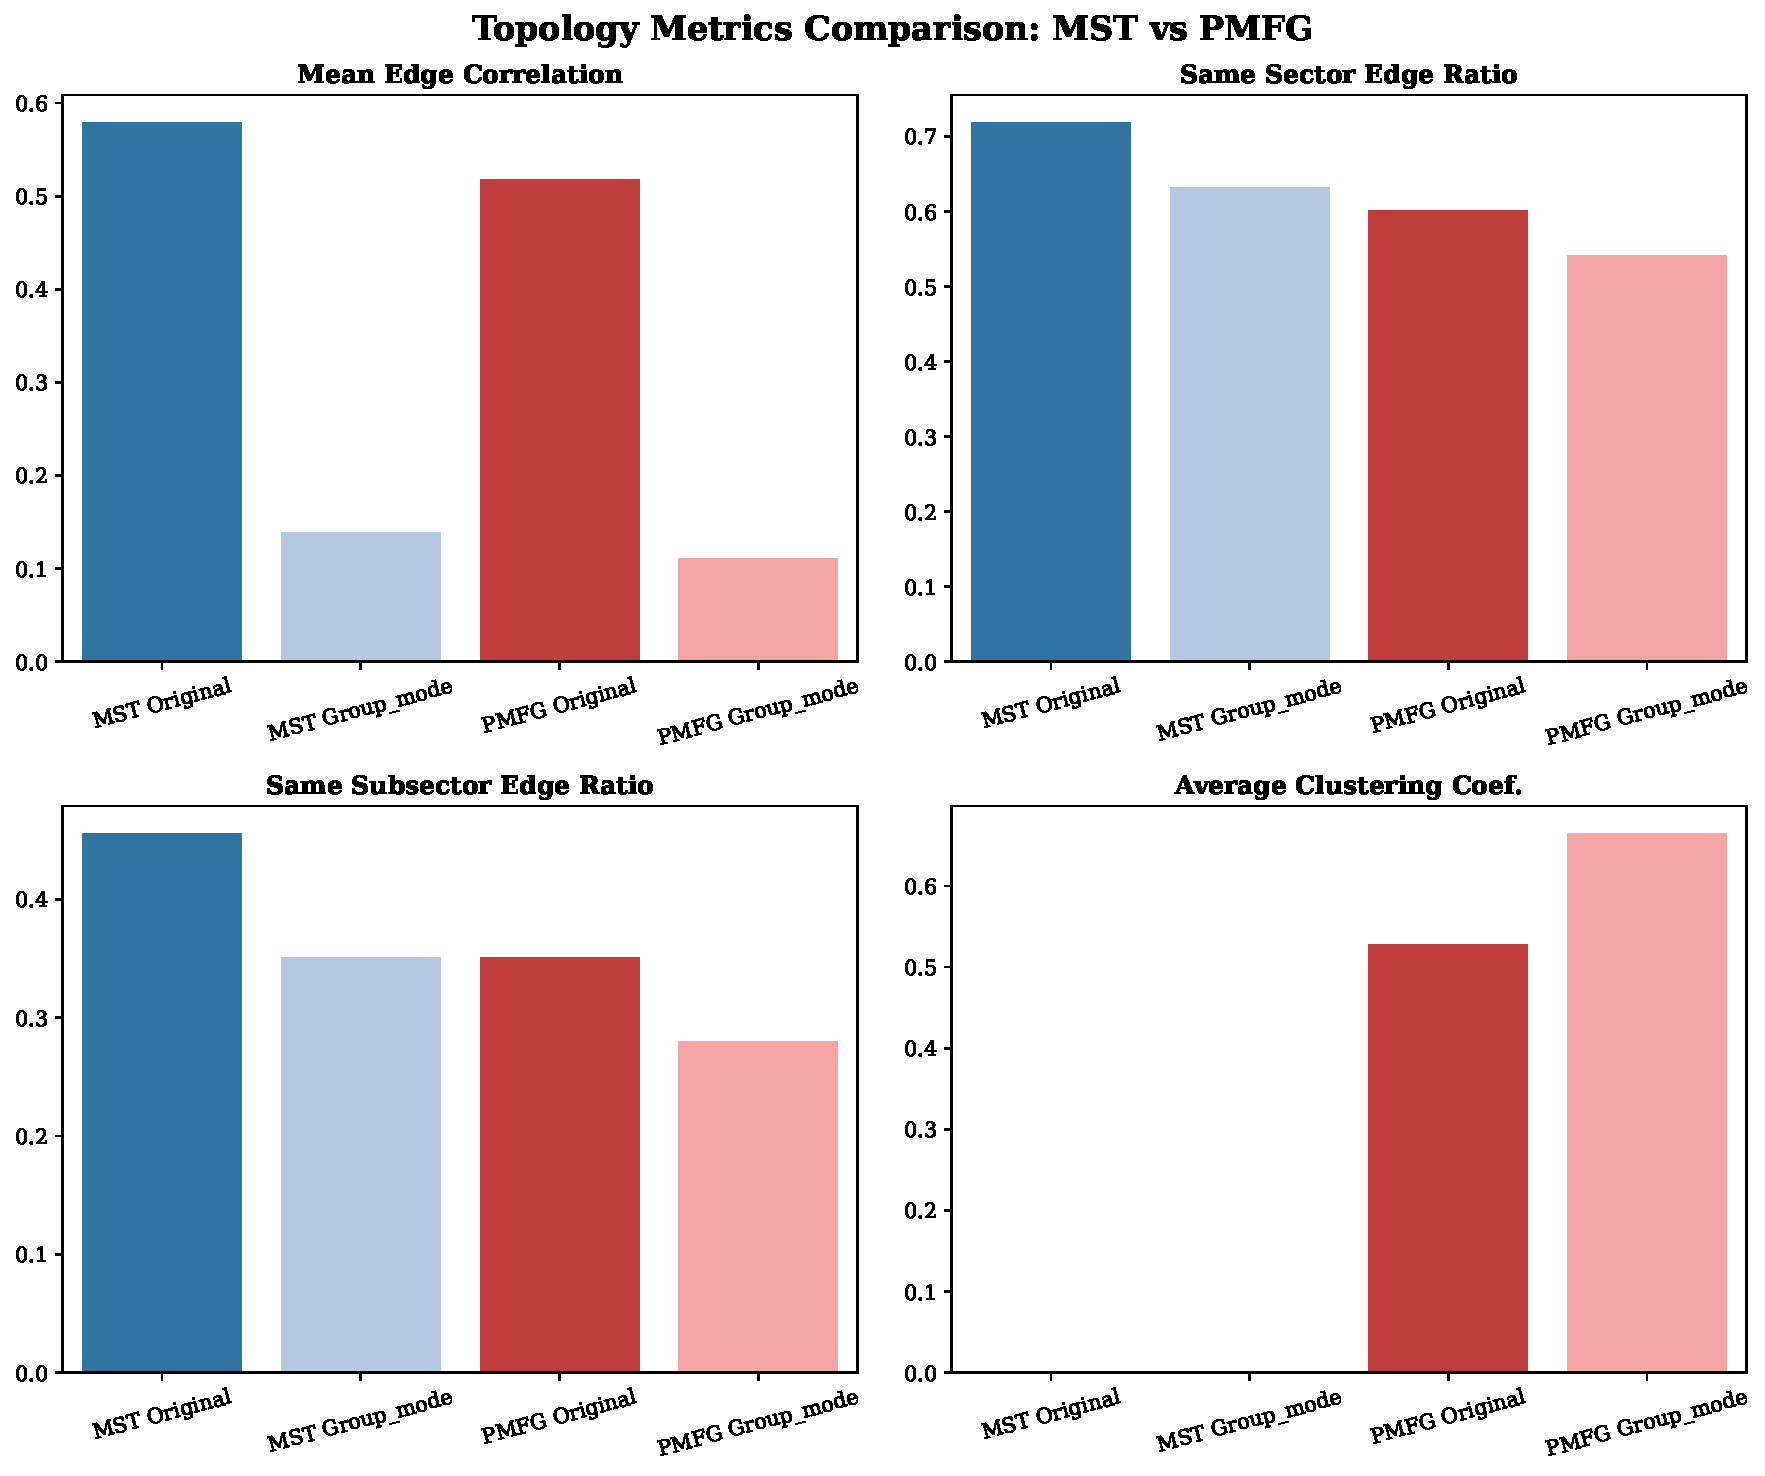
\includegraphics[width=\linewidth]{images/figure_13_network_topology_comparison.pdf}
\caption{Network topology comparison across original, filtered and group-mode MST/PMFG representations.}
\label{fig:network_topology}
\end{figure}
\FloatBarrier

The topology comparison supports a mesoscopic interpretation. Group-mode networks have lower mean edge correlations, but the PMFG clustering coefficient increases. Same-sector and same-subsector ratios remain substantial even after market-mode removal. This pattern is consistent with localized dependency structure rather than pure random residual noise. MST clustering is zero by construction because trees do not contain triangles; the PMFG clustering coefficient is therefore a distinctive advantage of the richer planar representation.

\begin{table}
\centering
\caption{PMFG clique and planarity diagnostics.}
\label{tab:pmfg_cliques}
\begin{tabular}{lrrrrl}
\toprule
Matrix & Nodes & Edges & Triangles & 4-cliques & Planar \\
\midrule
Original & 58 & 168 & 166 & 55 & Yes \\
Filtered & 58 & 168 & 166 & 55 & Yes \\
Group Mode & 58 & 168 & 166 & 55 & Yes \\
\bottomrule
\end{tabular}
\end{table}
\FloatBarrier

The clique counts are also construction checks. For a PMFG with 58 nodes, 168 edges are expected. The presence of 166 triangles and 55 4-cliques confirms that the PMFG contains richer local geometry than the MST. These local structures are precisely what can be transformed into network predictors for the forecasting experiment.

\subsection{Hub reorganization after RMT filtering}

Hub rankings reveal which assets act as bridges or local centers. Figure~\ref{fig:hub_rank} compares hub rankings before and after filtering. In the original PMFG, GGBR4 is the top betweenness node and BBDC4 is the top degree node. In the group-mode PMFG, GUAR3 becomes the leading node by both degree and betweenness.

\begin{figure}
\centering

\includegraphics[width=\linewidth]{images/figure_14_network_hub_rank_comparison.pdf}
\caption{Hub-rank comparison across original and group-mode networks. RMT filtering changes which assets act as central bridges in the dependency topology.}
\label{fig:hub_rank}
\end{figure}
\FloatBarrier

This hub shift is important. Original hubs can reflect market-wide correlation strength, liquidity and broad exposure. Group-mode hubs are more likely to represent localized bridges after the common component is removed. The appearance of assets such as GUAR3, BBDC3, VALE3, CCRO3, SAPR4 and CMIG3 in group-mode rankings suggests that RMT filtering changes the economic interpretation of centrality.
